\newpage
\section{System overview}
The system consists of a analog and a digital part. 

\subsection{Analog}

\begin{figure}[!htbp]
    \centering
    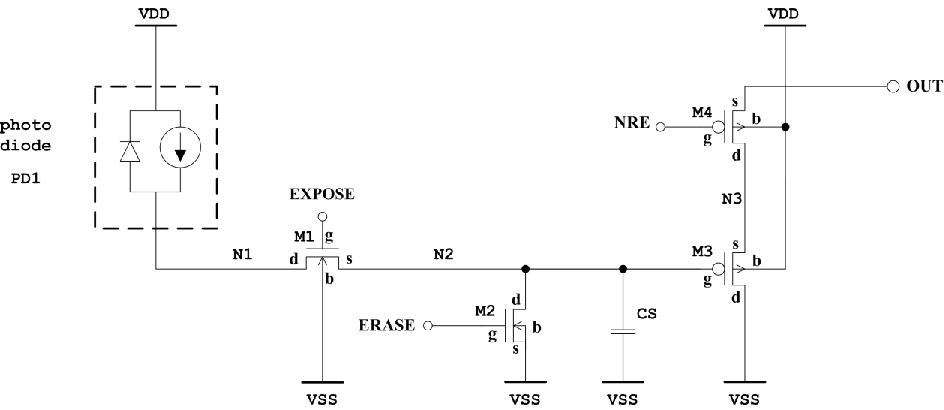
\includegraphics[width=\textwidth]{Images/Circuits/analog_circuit.pdf}
    \caption{Schematic of the analog readout part of the digital camera}
    \label{fig:system:an:sch}
\end{figure}

The analog part converts the electrons collected on the surface of the photodiode, in to an analog voltage. 
This voltage will charge up a capacitor depending on the lighting condition, for example low light condition will use longer time to charge capacitor. 
The expose transistor controls how  how long the capacitor can be charged for. 
The erase transistor controls the readout circuit so it does not overexpose the pixels. 
The two output transistors generate a current mirror which drives the output when a pixel is stored. 

To create a camera with more than one pixel, the pixels are connected in a matrix, shown in \cref{fig:app:fig:pixelarray} in \cref{fig:app:pixelarray}.

\subsection{Digital}

\begin{figure}[!htbp]
    \centering
    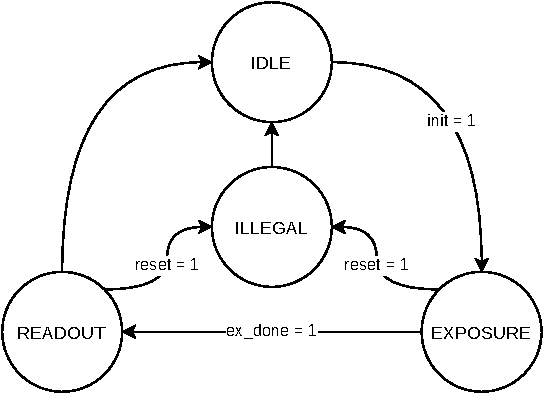
\includegraphics[width=0.7\textwidth]{Images/other/re_control_state.pdf}
    \caption{The different states of the control logic.}
    \label{fig:system:dig:states}
\end{figure}

The digital part controls the active pixel row, the exposure and the erase function of the analog part. 
%To obtain the required timing and the different states of capturing a picture, we use either a FPGA or an ASIC. 
%All three of these can be programmed by writing software with a HDL. 


From \cref{fig:system:dig:states} the four different states in the finite state machine (FSM) are presented. 
The FSM describes how the control logic captures a picture.
Starting with IDLE, the analog part is held stationary. 
When a picture is initialized, the state changes to EXPOSURE.
The pixels should be exposed for a set amount of time (until \texttt{ex\_done}, before continuing to the READOUT state. 
The READOUT consists of pulsing the pixel rows and controlling the ADC to read out the analog voltage to a digital value. 
After the readout is done, the state is set back to IDLE. 

The ILLEGAL state is used to reset the digital and analog parts, before going back to IDLE state.

All the timing of the FSM and states are synchronous, using a clock frequency of \SI{1}{\kilo\hertz}.